
CMEs

Another type of structure frequently found to be embedded in the slow and fast solar-wind streams are transient CMEs which have durations of a few days. CMEs make up about \SI{5}{\percent} of the solar wind's flow share during solar cycle minima, but can represent up to about \SI{50}{\percent} during solar cycle maxima \citep{Richardson2012}.\\

CMEs are eruptions of coronal magnetized plasma, which expand within hours to blobs with sizes of a few solar radii. They continuously expand further while moving farther away from the Sun into the heliosphere.\\

Long before the origins of magnetospheric disturbances were actually attributed to CMEs, the solar influence was identified as their source by \citet{Carrington1859}. Indeed, CMEs are the major drivers for strong geomagnetic disturbances, because they carry the most extreme conditions found in the solar wind. Thus, they are of major importance to space weather -- their impacts on the terrestrial magnetosphere are covered in the following \autoref{sec:space_weather}.\\

CMEs were detected in white-light observations made by the first space-based coronagraphs on board the OSO~7 satellite \citep{Tousey1973} and the Skylab space station \citep{MacQueen1974}. These observations show the steady outflow of solar wind, broken by intermittend ejections of coronal plasma. Subsequently, the kinematic properties of CMEs were identified from the white-light images \citep{MacQueen1980}. Now, coronagraphs observe the corona and hence CMEs continuously from the first Lagrange point in front of Earth with the SOHO spacecraft and from different equatorial perspectives with the STEREO~A and~B spacecraft. The image of the corona from 23~September 2012, made by the SECCHI/COR2 coronagraph onboard STEREO~A, shows a CME to the top right, see \autoref{fig:CME_COR2_0120923_182400_dbc2A}.\\
\begin{figure}[htb]
	\fcapside[\FBwidth]{
		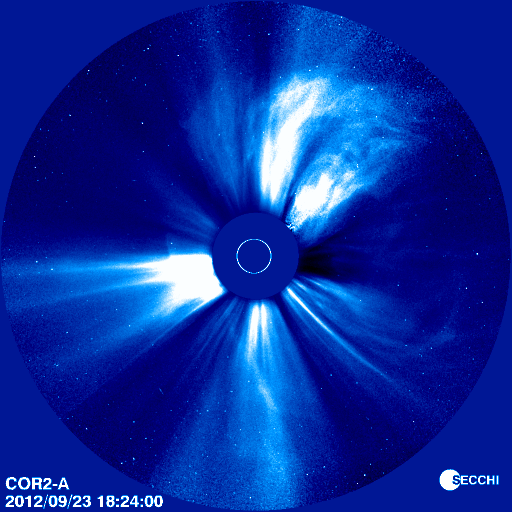
\includegraphics[width=0.6\textwidth]{figures_of_others/images/CME_COR2_0120923_182400_dbc2A.png}
	}{
		\caption{Image of the corona out to \SI{15}{\Rs} from 23~September 2012 made by the SECCHI/COR2 coronagraph onboard the STEREO~A spacecraft. The solar disk is covered by the occulter disk and its position is indicated by the white circle. The bright blob to the top right is the CME; the smooth elongated lines are solar wind streamers. Credit: NASA/STEREO... find optimal event... with shock and flux rope?}
		\label{fig:CME_COR2_0120923_182400_dbc2A}
	}
\end{figure}

It was early determined that solar ejecta should drive shock waves ahead \citep{Gold1962}. In fact, shocks with trailing low proton temperatures caused by fast CMEs were then found in in-situ measurements \citep{Gosling1973,Gosling1974}. \citet{Burlaga1981} analyzed magnetic field and plasma in-situ data from five spacecraft and identified a shock wave with a trailing turbulent sheath region followed by an organized helical magnetic structure that they called magnetic cloud (MC). MCs have an enhanced magnetic field, a smooth rotation in the azimuthal magnetic field component and they show low densities and temperatures \citep{Burlaga1981}. Thus, MCs have a low thermal to magnetic pressure ratio (i.e., a small plasma beta) and the magnetic field dominates the plasma. Furthermore, the overall pressure in MCs is higher than in the ambient solar wind, resulting in the expansion of MCs on their way out. Shock-driving CMEs containing a helical MC are actually identified with magnetic flux ropes that expand self-similarly and that remain in connection with the solar surface \citep{Chen1997}.\\

Three CMEs can be seen in the solar-wind measurements showed previously in \autoref{fig:ACE_64s_v7_thesis_CIRs_2013-5-1_65_plot}, passing by the ACE spacecraft at L1 on 24~May, 6~June, and 27~June in 2013. The latter CME is seen in detail in \autoref{fig:ACE_64s_v7_thesis_CME_2013-6-26_6_plot}, it has a fairly recognisable MC. In addition to the solar-wind in-situ parameters, I indicated the shock, compression zone and the MC with dotted lines, and plotted the geomagnetic \Kp{}~index in order to visualize the CME's impact on the magnetosphere. This MC contains a sector boundary and is trailed by an interaction region caused by the following HSS.\\
\begin{figure}[htb]
	\centering
	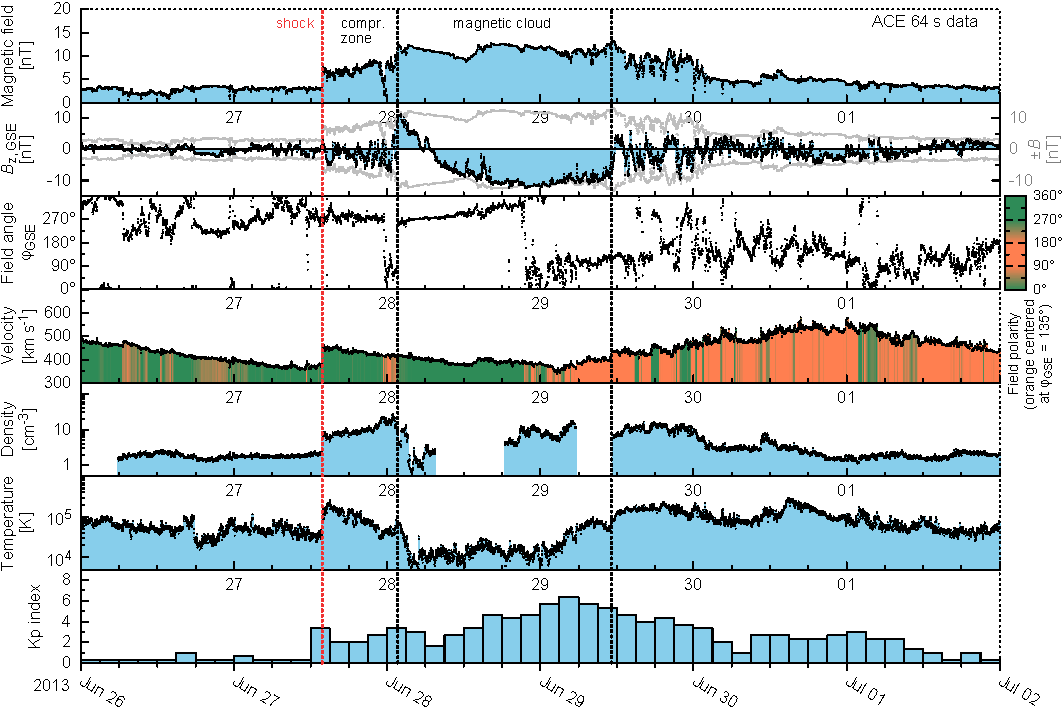
\includegraphics[width=\textwidth]{figures_of_mine/gnuplots/ACE_64s_v7_thesis_CME_2013-6-26_6_plot.pdf}
	\caption{Solar wind with a CME, measured at L1 during the time period 26~June to 2~July in 2013. The solar-wind parameters are the magnetic field strength, its z-component and ecliptic field angle in GSE~coordinates, the proton velocity, density, and temperature; in addition, the geomagnetic \Kp~index is plotted in the bottom panel. In the velocity panel also the field polarity is color coded -- assuming a Parker spiral angle of \SI{135}{\degree}. I indicated the shock, the compression zone, and the duration of the magnetic cloud with dotted lines. Blank periods indicate bad or missing data. The solar-wind data was measured with the MAG and SWEPAM instruments onboard the ACE spacecraft and is obtained from the ACE~Science~Center. The \Kp{}~data is obtained from the GFZ~Potsdam.}
	\label{fig:ACE_64s_v7_thesis_CME_2013-6-26_6_plot}
\end{figure}

The revelation that CMEs have always flux ropes \citep{Vourlidas2013} leads to the expansion of the CME definition based on white-light images made by \citet{Hundhausen1984}. \citet{Vourlidas2013,Vourlidas2014} include magnetic flux ropes in their CME redefinition: 'A CME is the eruption of a coherent magnetic, twist-carrying coronal structure with angular width of at least \SI{40}{\degree} and able to reach beyond \SI{10}{\Rs} which occurs on a time scale of a few minutes to several hours'.\\





%white-light shock
Disturbances in front of fast CMEs are identified as shocks in the white-light images of the newer SOHO coronagraph as well \citep{Sheeley2000}.


The shock itself is too narrow to be resolved by the coronagraph

the diffuse feature ahead of the void -- the flux rope -- is the shock sheath and the outer edge of this sheath is the shock location.

The brightness of the sheath region is caused by the density jump across the fast mode MHD shock.




shocks
their white-light and in-situ structure
in-situ figure

flux-ropes/MCs
definition
orientation
BSS


associated events
flares
SEPs

surface formation
acceleration
interaction



extreme events

CME forecast
- frequency
- CME models

open questions
- formation
- acceleration


figures
- coronagraph perspectives + maybe annotated
- in-situ
- flux rope

